\documentclass[12pt,a4paper]{article}

% ─── Page Layout ───────────────────────────────────────────────────────────────
\usepackage[a4paper, margin=0.8in, headheight=14pt]{geometry}

% ─── Fonts (XeLaTeX) ───────────────────────────────────────────────────────────
\usepackage{fontspec}
\usepackage{unicode-math}
\setmainfont{TeX Gyre Pagella}
\setmonofont[Scale=0.88]{TeX Gyre Cursor}
\setmathfont{Latin Modern Math}

% ─── Packages ──────────────────────────────────────────────────────────────────
\usepackage{xcolor}
\usepackage{colortbl}
\usepackage{titlesec}
\usepackage{enumitem}
\usepackage{tabularx}
\usepackage{longtable}
\usepackage{booktabs}
\usepackage{array}
\usepackage{amsmath}
\usepackage{tikz}
\usetikzlibrary{shapes.geometric, arrows.meta, positioning, calc, fit, decorations.pathreplacing, patterns}
\usepackage{tcolorbox}
\tcbuselibrary{skins, breakable}
\usepackage{hyperref}
\usepackage{fancyhdr}
\usepackage{graphicx}
\usepackage{microtype}
\hyphenpenalty=10000
\exhyphenpenalty=10000
\sloppy
\usepackage{caption}
\usepackage{setspace}
\usepackage{multirow}
\usepackage{tocloft}

% ─── Q&A helper ────────────────────────────────────────────────────────────────
\newcommand{\Q}[1]{\textbf{#1}\par\noindent\ignorespaces}

% ─── Colour Palette ────────────────────────────────────────────────────────────
\definecolor{myred}{RGB}{196,30,58}
\definecolor{mydark}{RGB}{30,30,50}
\definecolor{mygreen}{RGB}{14,120,80}
\definecolor{myteal}{RGB}{0,130,140}
\definecolor{myamber}{RGB}{180,100,0}
\definecolor{mypurple}{RGB}{100,30,160}
\definecolor{mygray}{RGB}{246,247,249}
\definecolor{mgframe}{RGB}{180,185,200}
\definecolor{watermark}{RGB}{145,150,170}
\definecolor{hdrred}{RGB}{250,232,235}
\definecolor{hdrgreen}{RGB}{220,244,233}
\definecolor{hdrteal}{RGB}{220,242,244}
\definecolor{hdramber}{RGB}{253,242,215}
\definecolor{hdrpurple}{RGB}{238,228,255}
\definecolor{hdrgray}{RGB}{238,240,245}

% ─── Section Formatting ────────────────────────────────────────────────────────
\titleformat{\section}
  {\large\bfseries\color{myred}}{\thesection.}{0.5em}{}
  [\vspace{1pt}{\color{myred}\rule{\linewidth}{0.8pt}}]
\titleformat{\subsection}
  {\normalsize\bfseries\color{myteal}}{\thesubsection}{0.5em}{}
\titlespacing*{\section}{0pt}{18pt}{7pt}
\titlespacing*{\subsection}{0pt}{11pt}{4pt}

% ─── Paragraph ─────────────────────────────────────────────────────────────────
\setlength{\parindent}{0pt}
\setlength{\parskip}{4pt}

% ─── TOC Styling ───────────────────────────────────────────────────────────────
\renewcommand{\cfttoctitlefont}{\large\bfseries\color{myred}}
\renewcommand{\cftaftertoctitle}{\par\noindent{\color{myred}\rule{\linewidth}{0.8pt}}}
\setlength{\cftbeforetoctitleskip}{0pt}
\setlength{\cftaftertoctitleskip}{6pt}
\renewcommand{\cftsecfont}{\normalsize\bfseries\color{mydark}}
\renewcommand{\cftsecpagefont}{\normalsize\bfseries\color{mydark}}
\renewcommand{\cftsecleader}{\cftdotfill{\cftdotsep}}
\setlength{\cftbeforesecskip}{7pt}
\renewcommand{\cftsubsecfont}{\small\color{mydark}}
\renewcommand{\cftsubsecpagefont}{\small\color{mydark}}
\setlength{\cftbeforesubsecskip}{3pt}
\setlength{\cftsubsecindent}{1.4em}

% ─── Table helpers ─────────────────────────────────────────────────────────────
\renewcommand{\arraystretch}{1.45}
\setlength{\tabcolsep}{6pt}
\arrayrulecolor{mydark}
\newcolumntype{B}[1]{>{\small\bfseries\raggedright\arraybackslash}m{#1}}
\newcolumntype{Y}{>{\small\raggedright\arraybackslash}X}
\renewcommand{\tabularxcolumn}[1]{m{#1}}

% ─── Header / Footer ───────────────────────────────────────────────────────────
\pagestyle{fancy}
\fancyhf{}
\fancyhead[L]{\small\color{myred}\textbf{BS-B401}\;\color{mydark}--- Biology for Engineers}
\fancyhead[R]{\small\color{myteal}\textbf{Module 5 Notes}}
\fancyfoot[C]{\small\color{mydark}\thepage}
\fancyfoot[R]{\small\color{watermark}\textit{\copyright\ Biraj Sarkar (CGEC)}}
\renewcommand{\headrulewidth}{0.5pt}
\renewcommand{\footrulewidth}{0.3pt}

% ─── Hyperref ──────────────────────────────────────────────────────────────────
\hypersetup{
  colorlinks=true, linkcolor=myteal, urlcolor=myteal,
  pdfauthor={Biraj Sarkar (CGEC)},
  pdftitle={BS-B401 --- Module 5 Notes: Enzymes}
}

% ─── tcolorbox styles ──────────────────────────────────────────────────────────
\tcbset{
  tikzbox/.style={
    colback=mygray, colframe=mgframe, boxrule=0.6pt, arc=4pt,
    left=8pt, right=8pt, top=6pt, bottom=6pt,
    colbacktitle=mgframe, coltitle=mydark, fonttitle=\small\bfseries
  },
  defbox/.style={
    colback=hdrgreen, colframe=mygreen, boxrule=0.8pt, arc=4pt,
    left=9pt, right=9pt, top=6pt, bottom=6pt,
    colbacktitle=mygreen, coltitle=white, fonttitle=\small\bfseries
  },
  formulabox/.style={
    colback=hdrteal, colframe=myteal, boxrule=0.8pt, arc=4pt,
    left=9pt, right=9pt, top=7pt, bottom=7pt,
    colbacktitle=myteal, coltitle=white, fonttitle=\small\bfseries
  },
  examplebox/.style={
    colback=hdramber, colframe=myamber, boxrule=0.8pt, arc=4pt,
    left=9pt, right=9pt, top=6pt, bottom=6pt,
    colbacktitle=myamber, coltitle=white, fonttitle=\small\bfseries
  },
  masonbox/.style={
    colback=hdrpurple, colframe=mypurple, boxrule=0.8pt, arc=4pt,
    left=9pt, right=9pt, top=6pt, bottom=6pt,
    colbacktitle=mypurple, coltitle=white, fonttitle=\small\bfseries
  },
  exambox/.style={
    colback=hdrpurple, colframe=mypurple, boxrule=1pt, arc=5pt,
    left=10pt, right=10pt, top=8pt, bottom=8pt,
    colbacktitle=mypurple, coltitle=white, fonttitle=\bfseries,
    breakable, title after break={\textbf{Frequently Asked / Viva Questions (contd.)}}
  }
}
\tcbset{breakable}
\tcbset{after={\par\color{black}}}

% ─── TikZ styles ───────────────────────────────────────────────────────────────
\tikzset{
  block/.style={rectangle, draw=myteal, fill=hdrteal,
    text width=2.4cm, align=center, minimum height=0.95cm,
    font=\small, rounded corners=3pt, line width=0.7pt},
  redblock/.style={rectangle, draw=myred, fill=hdrred,
    text width=2.4cm, align=center, minimum height=0.95cm,
    font=\small, rounded corners=3pt, line width=0.7pt},
  amberblock/.style={rectangle, draw=myamber, fill=hdramber,
    text width=2.4cm, align=center, minimum height=0.95cm,
    font=\small, rounded corners=3pt, line width=0.7pt},
  sumjunc/.style={circle, draw=myamber, fill=hdramber,
    minimum size=0.62cm, font=\small, line width=0.8pt},
  arrow/.style={-Stealth, thick, color=mydark},
  redarrow/.style={-Stealth, thick, color=myred},
  line/.style={thick, color=mydark}
}

\begin{document}

% ─── Title Page ───────────────────────────────────────────────────────────────
\begin{center}
  {\LARGE\bfseries\color{myred} BS-B401 --- Biology for Engineers}\\[5pt]
  {\normalsize\color{mydark} Semester IV \quad$\bullet$\quad 2L:1T:0P \quad$\bullet$\quad 3 Credits}\\[3pt]
  {\normalsize\color{myteal}\textbf{Module 5 Exam Notes: Enzymes}}\\[3pt]
  {\small\color{mydark} CGEC \;$|$\; B.Tech ECE (2023--27) \;$|$\; \textit{Biraj Sarkar}}
\end{center}
\vspace{2pt}
\noindent{\color{myred}\rule{\linewidth}{1.5pt}}
\vspace{2pt}

\hypersetup{linkcolor=mydark}
\tableofcontents
\hypersetup{linkcolor=myteal}
\newpage

\section{Enzymes}
\subsection{Catalysis and the active site}
\begin{tcolorbox}[defbox, title={Enzyme}]
An enzyme is a biological catalyst. It increases the rate at which a reaction approaches equilibrium by lowering the activation free-energy barrier. It does not change the reaction's overall free-energy difference or equilibrium constant. Most enzymes are proteins. Some RNAs also catalyse reactions.
\end{tcolorbox}

\begin{enumerate}[leftmargin=*, itemsep=3pt, topsep=4pt]
  \item \textbf{Bind.} Substrate binds in an active site through multiple interactions. In induced fit, binding shifts the conformations of enzyme and substrate.
  \item \textbf{Catalyse.} The site can orient reactants, stabilise the transition state, transfer protons, use a metal ion, or form a short-lived covalent intermediate.
  \item \textbf{Release.} Product leaves and the enzyme can act again. Binding the substrate very tightly alone does not guarantee rapid catalysis.
\end{enumerate}
\begin{tcolorbox}[examplebox, title={Two mechanisms with different chemical roles}]
\begin{itemize}[leftmargin=*, itemsep=3pt, topsep=4pt]
  \item \textbf{Lactase: hydrolysis.} It breaks the glycosidic bond in lactose to give glucose and galactose. Catalytic groups help transfer protons during cleavage. Water supplies the elements added across the broken bond.
  \item \textbf{Carbonic anhydrase: metal-assisted catalysis.} It accelerates reversible conversion of carbon dioxide and water into bicarbonate and a proton. A zinc ion helps activate bound water. The resulting hydroxide attacks carbon dioxide, followed by product release and regeneration of the active site.
\end{itemize}
\end{tcolorbox}

\subsection{Classification by reaction type}
\par\vspace{5pt}
\begingroup
\setlength{\extrarowheight}{1pt}
\noindent\begin{tabularx}{\linewidth}{|B{3.5cm}|Y|Y|}
\hline
\textbf{Class} & \textbf{Reaction} & \textbf{Example} \\ \hline
EC 1 Oxidoreductases & Transfer electrons or hydrogen. & Lactate dehydrogenase. \\ \hline
EC 2 Transferases & Transfer a functional group. & Hexokinase transfers a phosphoryl group. \\ \hline
EC 3 Hydrolases & Cleave bonds using water. & Lactase. \\ \hline
EC 4 Lyases & Cleave without hydrolysis or oxidation, or add groups to double bonds. & Aldolase. Carbonic anhydrase is a hydro-lyase. \\ \hline
EC 5 Isomerases & Rearrange atoms within a molecule. & Triose phosphate isomerase. \\ \hline
EC 6 Ligases & Join molecules, commonly coupled to nucleotide energy use. & Glutamine synthetase. \\ \hline
EC 7 Translocases & Catalyse movement across membranes or separation within membranes. & Sodium-potassium ATPase. \\ \hline
\end{tabularx}\par
\endgroup
\textbf{Classification source.} \href{https://iubmb.qmul.ac.uk/}{NC-IUBMB enzyme nomenclature}. Older classifications often list the first six classes.
\subsection{Monitoring a reaction}
\begin{itemize}[leftmargin=*, itemsep=3pt, topsep=4pt]
  \item \textbf{Measure a change.} Follow product appearance or substrate disappearance. Express initial rate in concentration per unit time.
  \item \textbf{Choose a signal.} An optical signal may follow absorbance, fluorescence or a coupled reporter reaction. A blank is used to distinguish background signal.
  \item \textbf{Interpret the slope.} Estimate $v_0$ from the initial nearly linear part, where substrate depletion and product effects are small. Record units and ensure the signal tracks the species of interest.
  \item \textbf{Compare like with like.} Enzyme amount, temperature, pH and measurement conditions matter when comparing the reported rates.
\end{itemize}
\section{Kinetics and Catalytic RNA}
\subsection{Michaelis--Menten equation and interpretation}
\begin{tcolorbox}[formulabox, title={Initial-rate model}]
For a simple one-substrate model, let $E+S\rightleftharpoons ES\to E+P$. Use rate constants $k_1$, $k_{-1}$ and $k_{\mathrm{cat}}$ in that order. Assume early times, an approximately steady $ES$ concentration and negligible reverse reaction from product.
\[
0\approx k_1([E]_T-[ES])[S]-(k_{-1}+k_{\mathrm{cat}})[ES].
\]
Rearrange and substitute $v_0=k_{\mathrm{cat}}[ES]$:
\[
\begin{aligned}
K_m&=\frac{k_{-1}+k_{\mathrm{cat}}}{k_1},&
[ES]&=\frac{[E]_T[S]}{K_m+[S]},\\
V_{\max}&=k_{\mathrm{cat}}[E]_T,&
v_0&=\frac{V_{\max}[S]}{K_m+[S]} .
\end{aligned}
\]
\end{tcolorbox}

\begin{tcolorbox}[tikzbox, title={Substrate saturation in a simple initial-rate model}]
\centering
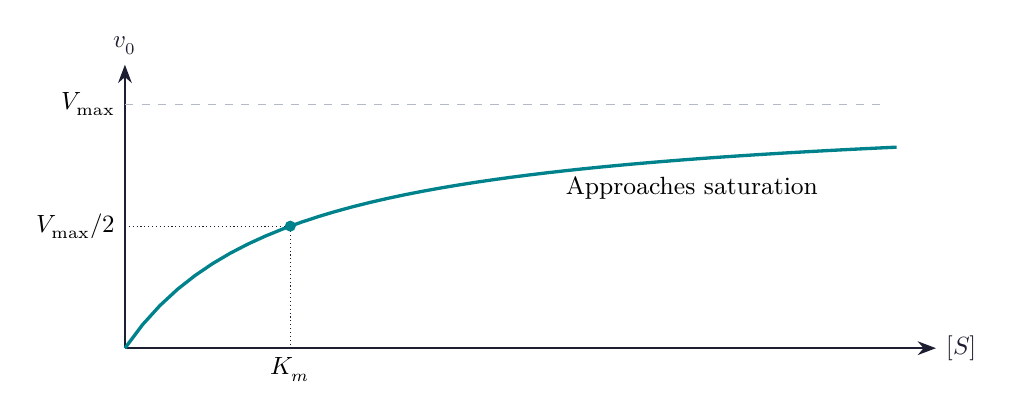
\begin{tikzpicture}[every node/.style={font=\small}]
\draw[arrow] (0,0)--(10.3,0) node[right] {$[S]$};
\draw[arrow] (0,0)--(0,3.6) node[above] {$v_0$};
\draw[myteal,very thick,domain=0:9.8,samples=45] plot (\x,{3.1*\x/(2.1+\x)});
\draw[mgframe,dashed] (0,3.1)--(9.7,3.1);
\draw[mydark,densely dotted] (0,1.55)--(2.1,1.55)--(2.1,0);
\fill[myteal] (2.1,1.55) circle (2pt);
\node[left] at (0,3.1) {$V_{\max}$};
\node[left] at (0,1.55) {$V_{\max}/2$};
\node[below] at (2.1,0) {$K_m$};
\node[below] at (7.2,2.30) {Approaches saturation};
\end{tikzpicture}\par
\end{tcolorbox}

\begin{itemize}[leftmargin=*, itemsep=3pt, topsep=4pt]
  \item \textbf{Units.} $K_m$ is concentration, $V_{\max}$ is concentration per time, and $k_{\mathrm{cat}}$ is inverse time.
  \item \textbf{At half saturation.} $[S]=K_m$ gives $v_0=V_{\max}/2$. It is not generally a pure binding affinity.
  \item \textbf{At low substrate.} $v_0\approx(k_{\mathrm{cat}}/K_m)[E]_T[S]$. The ratio compares catalytic efficiency in the low-substrate limit.
  \item \textbf{Why measure parameters?} They help compare biological reactions, predict rate at a given substrate level, and distinguish reduced turnover from altered apparent substrate dependence.
\end{itemize}
\begin{tcolorbox}[examplebox, title={Calculate rate and turnover}]
If $V_{\max}=12\,\mu\mathrm{M\,s^{-1}}$ and $K_m=3\,\mathrm{mM}$, then at $[S]=6\,\mathrm{mM}$ the rate is $12(6)/(3+6)=8\,\mu\mathrm{M\,s^{-1}}$. If $[E]_T=0.20\,\mu\mathrm M$, the turnover number is $12/0.20=60\,\mathrm{s^{-1}}$.
\end{tcolorbox}

\subsection{Interpret enzyme measurements and common rate changes}
\begin{tcolorbox}[examplebox, title={Convert a time trace into an initial rate}]
In an illustrative measurement, product rises from $2$ to $8\,\mu\mathrm M$ in the first $3\,\mathrm s$ with an approximately straight trace. The initial rate estimate is $(8-2)/3=2\,\mu\mathrm{M\,s^{-1}}$. If the curve later bends, averaging over the entire trace may give a different value. Report the early slope and the units used for concentration and time.
\end{tcolorbox}

\par\vspace{6pt}
\noindent\begin{tabularx}{\linewidth}{|B{3.3cm}|Y|Y|}
\hline
\textbf{Change} & \textbf{Expected result in the simple model} & \textbf{Reason} \\ \hline
More enzyme at the same substrate level & $V_{\max}$ increases with $[E]_T$ while $K_m$ is unchanged. & There are more catalytic sites. Each site follows the same model. \\ \hline
More substrate at fixed enzyme level & The initial rate approaches $V_{\max}$. & Most active sites are occupied at high substrate. \\ \hline
Ideal competitive inhibition & Apparent $K_m$ rises while $V_{\max}$ stays the same. & Substrate and inhibitor compete for free enzyme. \\ \hline
Pure noncompetitive inhibition & Apparent $V_{\max}$ falls while $K_m$ stays the same. & This ideal special case reduces usable catalytic capacity. Other mixed inhibition patterns can affect both quantities. \\ \hline
\end{tabularx}\par

\begin{tcolorbox}[masonbox, title={Connect structure to the kinetics}]
A low value of $K_m$ means half-maximal rate is reached at a lower substrate concentration under the stated model. It is not automatically a binding constant. Compare $k_{\mathrm{cat}}$ when the question is about turnover per active site, and $k_{\mathrm{cat}}/K_m$ for the low-substrate limit.
\end{tcolorbox}

\subsection{RNA catalysis}
\begin{tcolorbox}[defbox, title={Ribozyme}]
A ribozyme is a folded RNA that catalyses a reaction. Its shape positions substrates and reactive groups. Some catalytic RNAs depend on associated ions or proteins.
\end{tcolorbox}

RNase P has a catalytic RNA component involved in processing precursor tRNAs in many organisms. The ribosomal RNA at the large-subunit catalytic centre participates in peptide-bond formation. These examples connect information-processing molecules with chemical catalysis.

\subsection{Explain how RNA can act as a catalyst}
\begin{itemize}[leftmargin=*, itemsep=2pt]
  \item \textbf{Fold.} Base pairing and tertiary contacts bring reactive groups into a definite three-dimensional arrangement.
  \item \textbf{Position.} Folded RNA can bring reactants together and orient them. Metal ions can help stabilise charge in some ribozymes.
  \item \textbf{Illustrate.} RNase P processes precursor tRNA, a self-splicing intron can promote its own removal, and the ribosomal catalytic centre participates in peptide-bond formation. These examples show distinct catalytic roles for RNA.
\end{itemize}

\textbf{Reading.} \href{https://iubmb.qmul.ac.uk/kinetics/}{IUBMB kinetic terminology} and \href{https://www.nobelprize.org/uploads/2018/06/cech-lecture.pdf}{Cech's lecture on RNA catalysis}.

\newpage
\begin{center}
  {\large\bfseries\color{myred} Quick Revision --- Module 5}\\[3pt]
  {\small\color{mydark} Enzymes $|$ BS-B401}
\end{center}
\noindent{\color{myred}\rule{\linewidth}{1.2pt}}\par\vspace{4pt}

\begin{tcolorbox}[formulabox, title={Key Concepts at a Glance}]
\renewcommand{\arraystretch}{1.35}
\noindent\begin{tabularx}{\linewidth}{B{4.5cm}Y}
Michaelis--Menten & $v_0=V_{\max}[S]/(K_m+[S])$. \\[3pt]
Half-maximal velocity & $[S]=K_m$ gives $v_0=V_{\max}/2$. \\[3pt]
Turnover & $k_{\mathrm{cat}}=V_{\max}/[E]_T$. \\[3pt]
\end{tabularx}\par
\end{tcolorbox}

\begin{tcolorbox}[defbox, title={One-Line Definitions}]
\begin{itemize}[leftmargin=*, itemsep=3pt, topsep=4pt]
  \item \textbf{Active site.} Region that binds substrate and supports catalysis.
  \item \textbf{Initial rate.} Early slope of product formation or substrate disappearance.
  \item \textbf{Ribozyme.} Catalytic RNA.
\end{itemize}
\end{tcolorbox}

\begin{tcolorbox}[exambox, title={Frequently Asked / Viva Questions}]
\begin{enumerate}[topsep=0pt, label=\textbf{Q\arabic*.}, itemsep=5pt, leftmargin=*]
  \item \Q{What barrier does an enzyme lower?}
    The activation free-energy barrier.
  \item \Q{Does an enzyme change equilibrium?}
    It changes the approach rate. Equilibrium is set by energetics.
  \item \Q{What is induced fit?}
    Binding changes or selects conformations suited to catalysis.
  \item \Q{What reaction does lactase catalyse?}
    Hydrolysis of lactose to glucose and galactose.
  \item \Q{What supports catalysis in carbonic anhydrase?}
    A zinc ion helps activate water.
  \item \Q{What variable is monitored to determine a rate?}
    A signal that tracks product formation or substrate loss.
  \item \Q{Why use initial rate?}
    Little product has built up and substrate depletion is small.
  \item \Q{What are the units of turnover number?}
    Inverse time.
  \item \Q{Which new class involves membrane movement?}
    Translocases, EC 7.
  \item \Q{Give one example of catalytic RNA.}
    The RNA component of RNase P.
\end{enumerate}
\end{tcolorbox}

\begin{tcolorbox}[tikzbox, title={Summary Comparison}]
\par\vspace{5pt}
\begingroup
\setlength{\extrarowheight}{1pt}
\noindent\begin{tabularx}{\linewidth}{|B{3.45cm}|Y|Y|}
\hline
\textbf{Feature} & \textbf{Protein enzyme} & \textbf{Ribozyme} \\ \hline
Catalytic component & Folded polypeptide. & Folded RNA. \\ \hline
Examples & Lactase or carbonic anhydrase. & RNase P RNA or catalytic ribosomal RNA. \\ \hline
\end{tabularx}\par
\endgroup
\end{tcolorbox}

\end{document}
